\documentclass[12pt,a4paper]{book}
\usepackage[utf8]{inputenc}
\usepackage[T1]{fontenc}
\usepackage[french]{babel}
\usepackage{graphicx}
\usepackage{booktabs}
\usepackage{amsmath}
\usepackage{amssymb}
\usepackage{geometry}
\usepackage{float}
\usepackage{caption}
\usepackage{subcaption}
\usepackage{fancyhdr}
\usepackage{setspace}
\usepackage{titlesec}
\usepackage{chngcntr}
\usepackage[table]{xcolor}   % xcolor inclut déjà "color" ET l'option [table] remplace colortbl
\usepackage{array}
\usepackage{multirow}        % <-- MANQUAIT : nécessaire pour \multirow
\usepackage{longtable}
\usepackage{gensymb}
\usepackage{hyperref}        % <-- hyperref doit être chargé en dernier (ou presque)

% --- SUPPRESSION DES PAGES VIDES ---
\let\cleardoublepage\clearpage

% Configuration de la page
\geometry{
	a4paper,
	left=2.5cm,
	right=2.5cm,
	top=2.5cm,
	bottom=2.5cm
}

% Configuration des en-têtes et pieds de page
\pagestyle{fancy}
\fancyhf{}
\fancyhead[LE,RO]{\leftmark}
\fancyfoot[CE,CO]{\thepage}
\renewcommand{\headrulewidth}{0.4pt}

% Configuration des titres de chapitres
\titleformat{\chapter}[hang]{\Huge\bfseries}{}{0pt}{}
\titlespacing*{\chapter}{0pt}{-20pt}{20pt}

% Numérotation des figures par chapitre
\counterwithin{figure}{chapter}
\counterwithin{table}{chapter}

% Informations du livre
\title{
	\begin{center}
		
\includegraphics[width=1.1in,height=1.1in]{./logo/Logo_fac_science}
		\hspace{9cm}
		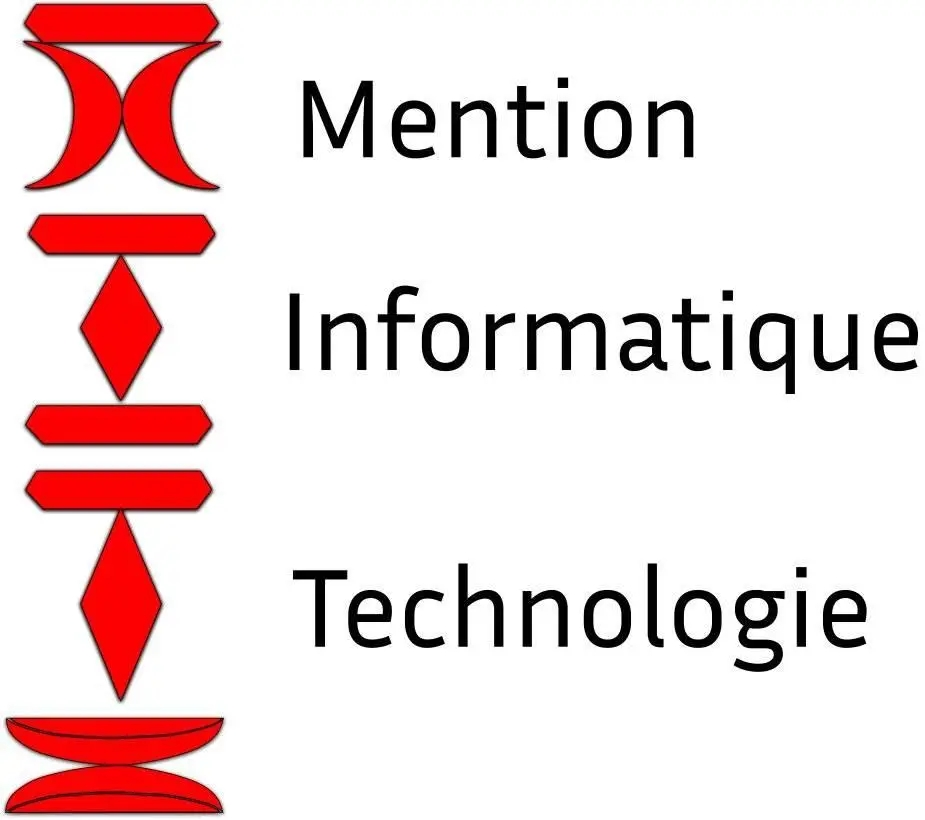
\includegraphics[width=1.1in,height=1.1in]{./logo/logo_MIT}
	\end{center}
	\vspace{-2.5cm}
	\textbf{\textit{
			Université d'Antananarivo\\[12pt]
			Faculté des Sciences\\[15pt] 
			Mention Informatique et Technologie (MIT)}\\[50pt]} \bigskip
	\textsc{grade : \textbf{Master 1 }\\[2pt]}
	Parcours: \textsc{\textbf{Innovation et Technologie (INT)}} 
	
	\vfill	
	\rule{0.75\textwidth}{3pt} \vspace{10pt}
	\textbf{\\ANALYSE FACTORIELLE DES CORRESPONDANCES SUR R :\\
		\Large \textbf{Étude des Loisirs selon la Profession}}
	\rule{0.75\textwidth}{3pt}
	\vfill
}

\date{\today \\[25pt]
	\textit{\textbf{Année universitaire : 2025 - 2026}}
}
\author{\underline{Nom:}\\[4pt]
	\textbf{RABESIHARISON Tolotraniaina Henri}\\[1.5pt] 
}

\begin{document}
	
	% --- TABLE DES MATIÈRES ---
	\pagenumbering{gobble}
	\maketitle
	\cleardoublepage
	\pagenumbering{roman}
	\addcontentsline{toc}{section}{Table des matières}
	\tableofcontents
	\cleardoublepage
	
	\pagenumbering{arabic}
	
	% --- PRÉFACE ---
	\chapter*{Préface}
	\addcontentsline{toc}{chapter}{Préface}
	\markboth{Préface}{Préface}
	
	\vspace{0.5cm}
	
	Ce livre propose une analyse statistique des loisirs selon la profession à travers l'\textbf{Analyse Factorielle des Correspondances (AFC)}. 
	
	L'étude porte sur \textbf{8 professions} et \textbf{12 loisirs} :
	
	\begin{itemize}
		\item \textbf{Professions} : Ouvrier, Employé, Cadre, Agriculteur, Étudiant, Retraité, Chômeur, Commerçant
		\item \textbf{Loisirs} : Cinéma, Sport, Lecture, Restaurant, Musée, Voyage, Jardinage, Bricolage, Jeux Vidéo, Cuisine, Danse, Photo
	\end{itemize}
	
	\vspace{0.3cm}
	
	L'objectif est de :
	\begin{itemize}
		\item Visualiser les relations entre les professions et les loisirs.
		\item Identifier les profils types de chaque profession.
		\item Comprendre les facteurs qui différencient les catégories socioprofessionnelles.
	\end{itemize}
	
	\vspace{0.3cm}
	
	Ce document s'adresse aux étudiants et professionnels souhaitant découvrir l'AFC à travers un cas pratique concret.
	
	\vspace{0.3cm}
	
	
	
	% --- CHAPITRE 1 : INTRODUCTION ---
	\chapter{Introduction}
	\markboth{Introduction}{Introduction}
	
	\section{Contexte de l'étude}
	
	Les loisirs occupent une place importante dans la vie quotidienne et varient considérablement selon la profession, le niveau de vie et l'environnement social. Comprendre ces différences permet de mieux appréhender les inégalités culturelles et sociales.
	
	\vspace{0.5cm}
	
	Dans ce contexte, il est essentiel de comprendre :
	\begin{itemize}
		\item \textbf{Quels loisirs sont associés à quelles professions ?}
		\item \textbf{Existe-t-il des oppositions structurantes entre les pratiques culturelles ?}
		\item \textbf{Quels sont les profils types de chaque catégorie socioprofessionnelle ?}
	\end{itemize}
	
	\section{Présentation des données}
	
	L'étude porte sur \textbf{8 professions} et \textbf{12 loisirs}. Le tableau ci-dessous présente les données collectées :
	
	\vspace{0.5cm}
	
	\begin{table}[H]
		\centering
		\caption{Tableau de contingence - Loisirs selon la Profession}
		\small
		\begin{tabular}{lrrrrrrrrrrrr}
			\toprule
			\textbf{Profession} & \textbf{Cinéma} & \textbf{Sport} & \textbf{Lecture} & \textbf{Restaurant} & \textbf{Musée} & \textbf{Voyage} & \textbf{Jardinage} & \textbf{Bricolage} & \textbf{JeuxVidéo} & \textbf{Cuisine} & \textbf{Danse} & \textbf{Photo} \\
			\midrule
			Ouvrier & 45 & 52 & 12 & 18 & 5 & 8 & 15 & 35 & 28 & 10 & 6 & 4 \\
			Employé & 38 & 32 & 28 & 25 & 15 & 20 & 18 & 22 & 20 & 18 & 12 & 10 \\
			Cadre & 25 & 18 & 52 & 35 & 42 & 48 & 30 & 25 & 8 & 30 & 15 & 28 \\
			Agriculteur & 10 & 15 & 8 & 6 & 3 & 5 & 55 & 42 & 2 & 8 & 4 & 3 \\
			Étudiant & 62 & 45 & 25 & 20 & 12 & 35 & 8 & 10 & 58 & 12 & 25 & 18 \\
			Retraité & 15 & 12 & 48 & 20 & 38 & 32 & 52 & 40 & 3 & 35 & 8 & 22 \\
			Chômeur & 30 & 18 & 20 & 12 & 10 & 8 & 15 & 12 & 40 & 25 & 10 & 6 \\
			Commerçant & 20 & 15 & 18 & 45 & 12 & 10 & 12 & 8 & 10 & 15 & 8 & 5 \\
			\bottomrule
		\end{tabular}
	\end{table}
	
	\section{Objectifs de l'étude}
	
	Les objectifs principaux de cette analyse sont :
	
	\begin{enumerate}
		\item \textbf{Identifier les relations} entre les professions et les loisirs pratiqués.
		\item \textbf{Déterminer les facteurs} qui différencient le plus les catégories socioprofessionnelles.
		\item \textbf{Classifier} les professions selon leurs pratiques de loisirs.
		\item \textbf{Évaluer la qualité} de l'analyse statistique.
	\end{enumerate}
	
	\section{Structure du rapport}
	
	Ce rapport est structuré en six chapitres :
	
	\begin{enumerate}
		\item \textbf{Introduction} : Présentation du contexte, des données et des objectifs.
		\item \textbf{Méthodologie} : Explication de l'Analyse Factorielle des Correspondances.
		\item \textbf{Carte factorielle des loisirs} : Analyse des relations entre loisirs.
		\item \textbf{Carte factorielle des professions} : Profils types des professions.
		\item \textbf{Biplot conjoint} : Relations croisées professions-loisirs.
		\item \textbf{Valeurs propres} : Qualité et fiabilité de l'analyse.
	\end{enumerate}
	
	% --- CHAPITRE 2 : MÉTHODOLOGIE ---
	\chapter{Méthodologie}
	\markboth{Méthodologie}{Méthodologie}
	
	\section{L'Analyse Factorielle des Correspondances (AFC)}
	
	L'\textbf{Analyse Factorielle des Correspondances} est une méthode statistique multidimensionnelle spécifique aux tableaux de contingence. Elle permet de :
	
	\begin{itemize}
		\item \textbf{Réduire} la dimensionnalité des données.
		\item \textbf{Visualiser} les relations entre les lignes et les colonnes.
		\item \textbf{Identifier} les associations préférentielles entre modalités.
	\end{itemize}
	
	\subsection{Principe de l'AFC}
	
	L'AFC transforme un tableau de contingence en représentations simultanées des lignes et des colonnes dans un espace de faible dimension. Elle repose sur la notion de \textbf{profil} :
	
	\begin{itemize}
		\item Chaque ligne (profession) est un profil de loisirs.
		\item Chaque colonne (loisir) est un profil de professions.
		\item L'analyse cherche à représenter au mieux les distances entre ces profils.
	\end{itemize}
	
	\vspace{0.5cm}
	
	\begin{center}
		\fbox{
			\begin{minipage}{0.8\textwidth}
				\textbf{Formule mathématique :}
				
				La distance du $\chi^2$ entre deux profils $i$ et $i'$ est :
				
				\[
				d^2(i,i') = \sum_{j=1}^{p} \frac{1}{n_{.j}} \left( \frac{n_{ij}}{n_{i.}} - \frac{n_{i'j}}{n_{i'.}} \right)^2
				\]
				
				Où $n_{ij}$ est l'effectif de la cellule $(i,j)$.
			\end{minipage}
		}
	\end{center}
	
	\subsection{Étapes de l'AFC}
	
	Le processus d'analyse se déroule en plusieurs étapes :
	
	\begin{enumerate}
		\item \textbf{Calcul des profils} lignes et colonnes.
		\item \textbf{Calcul de la matrice de distance du $\chi^2$}.
		\item \textbf{Extraction des valeurs propres et des vecteurs propres}.
		\item \textbf{Calcul des coordonnées} des lignes et des colonnes.
		\item \textbf{Interprétation des résultats}.
	\end{enumerate}
	
	\section{Description des variables}
	
	Le tableau ci-dessous présente les modalités utilisées dans cette étude :
	
	\begin{table}[H]
		\centering
		\caption{Description des modalités}
		\begin{tabular}{lcp{8cm}}
			\toprule
			\textbf{Type} & \textbf{Modalité} & \textbf{Description} \\
			\midrule
			\multirow{8}{*}{Professions} & Ouvrier & Travailleur manuel, secteur industriel \\
			& Employé & Travailleur tertiaire, bureau \\
			& Cadre & Profession intellectuelle supérieure \\
			& Agriculteur & Travailleur du secteur agricole \\
			& Étudiant & Personne en formation \\
			& Retraité & Personne âgée, hors activité \\
			& Chômeur & Personne sans emploi \\
			& Commerçant & Profession libérale, commerce \\
			\midrule
			\multirow{12}{*}{Loisirs} & Cinéma & Activité culturelle grand public \\
			& Sport & Activité physique \\
			& Lecture & Activité intellectuelle \\
			& Restaurant & Sortie gastronomique \\
			& Musée & Visite culturelle \\
			& Voyage & Découverte et dépaysement \\
			& Jardinage & Activité de plein air \\
			& Bricolage & Activité manuelle \\
			& Jeux Vidéo & Divertissement numérique \\
			& Cuisine & Activité culinaire \\
			& Danse & Activité artistique \\
			& Photo & Activité créative \\
			\bottomrule
		\end{tabular}
	\end{table}
	
	\section{Justification de l'AFC pour cette étude}
	
	L'AFC est particulièrement adaptée à cette étude car :
	
	\begin{itemize}
		\item Les données sont sous forme de \textbf{tableau de contingence}.
		\item Nous cherchons à \textbf{visualiser} simultanément les lignes et les colonnes.
		\item Nous voulons \textbf{identifier} des associations préférentielles.
		\item La distance du $\chi^2$ est spécifiquement adaptée aux profils.
	\end{itemize}
	
	% --- CHAPITRE 3 : CARTE FACTORIELLE DES LOISIRS ---
	\chapter{Carte Factorielle des Loisirs}
	\markboth{Carte Factorielle des Loisirs}{Carte Factorielle des Loisirs}
	
	\section{Présentation du graphique}
	
	La carte factorielle des loisirs permet de visualiser les \textbf{relations entre les différents loisirs} et leur positionnement dans l'espace défini par les axes principaux.
	
	\begin{figure}[H]
		\centering
		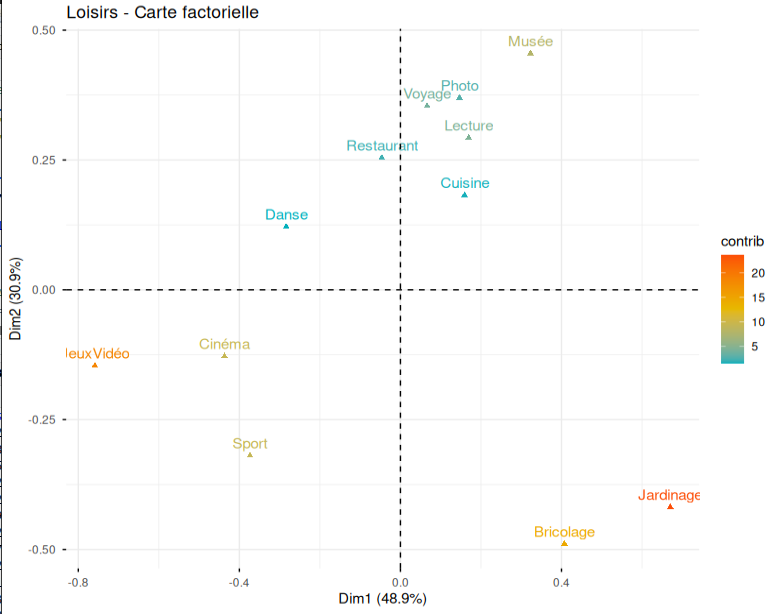
\includegraphics[width=0.85\textwidth]{./img/losirs_carte_factorielle.png}
		\caption{Carte factorielle des loisirs - Projection sur les axes 1 et 2}
		\label{fig:loisirs}
	\end{figure}
	
	\section{Interprétation des axes}
	
	\subsection{Axe horizontal (Dimension 1 - 48.9\%)}
	
	L'axe horizontal est l'axe principal qui explique \textbf{48.9\%} de l'inertie totale.
	
	\begin{itemize}
		\item \textbf{À droite} de l'axe : Loisirs \textbf{culturels et intellectuels} :
		\begin{itemize}
			\item \textcolor{blue}{Lecture}
			\item \textcolor{blue}{Musée}
			\item \textcolor{blue}{Voyage}
			\item \textcolor{blue}{Photo}
		\end{itemize}
		
		\item \textbf{À gauche} de l'axe : Loisirs \textbf{populaires et divertissants} :
		\begin{itemize}
			\item \textcolor{red}{Cinéma}
			\item \textcolor{red}{Sport}
			\item \textcolor{red}{Jeux Vidéo}
		\end{itemize}
	\end{itemize}
	
	\subsection{Axe vertical (Dimension 2 - 30.9\%)}
	
	L'axe vertical explique \textbf{30.9\%} de l'inertie totale. Il permet de distinguer :
	
	\begin{itemize}
		\item \textbf{Haut} : Loisirs \textbf{artistiques et créatifs} :
		\begin{itemize}
			\item \textcolor{orange}{Danse}
			\item \textcolor{orange}{Photo}
		\end{itemize}
		
		\item \textbf{Bas} : Loisirs \textbf{manuels et domestiques} :
		\begin{itemize}
			\item \textcolor{brown}{Bricolage}
			\item \textcolor{brown}{Jardinage}
		\end{itemize}
	\end{itemize}
	
	\section{Regroupement des loisirs}
	
	\begin{table}[H]
		\centering
		\caption{Regroupements des loisirs identifiés}
		\begin{tabular}{p{4cm}p{4cm}p{4cm}}
			\toprule
			\textbf{Culturel/Intellectuel} & \textbf{Divertissement/Populaire} & \textbf{Manuel/Domestique} \\
			\midrule
			Lecture & Cinéma & Jardinage \\
			Musée & Sport & Bricolage \\
			Voyage & Jeux Vidéo & Cuisine \\
			Photo & Restaurant & \\
			\bottomrule
		\end{tabular}
	\end{table}
	
	\section{Conclusion du chapitre}
	
	La carte factorielle des loisirs met clairement en évidence \textbf{trois groupes distincts} :
	
	\begin{enumerate}
		\item Un groupe \textcolor{blue}{culturel et intellectuel} (Lecture, Musée, Voyage, Photo)
		\item Un groupe \textcolor{red}{populaire et divertissant} (Cinéma, Sport, Jeux Vidéo)
		\item Un groupe \textcolor{brown}{manuel et domestique} (Jardinage, Bricolage, Cuisine)
	\end{enumerate}
	
	Ces groupes sont fortement opposés le long des axes principaux, ce qui indique des \textbf{pratiques culturelles différenciées} selon les catégories socioprofessionnelles.
	
	% --- CHAPITRE 4 : CARTE FACTORIELLE DES PROFESSIONS ---
	\chapter{Carte Factorielle des Professions}
	\markboth{Carte Factorielle des Professions}{Carte Factorielle des Professions}
	
	\section{Présentation du graphique}
	
	La carte factorielle des professions permet de visualiser la \textbf{position de chaque profession} dans l'espace défini par les axes principaux.
	
	\begin{figure}[H]
		\centering
		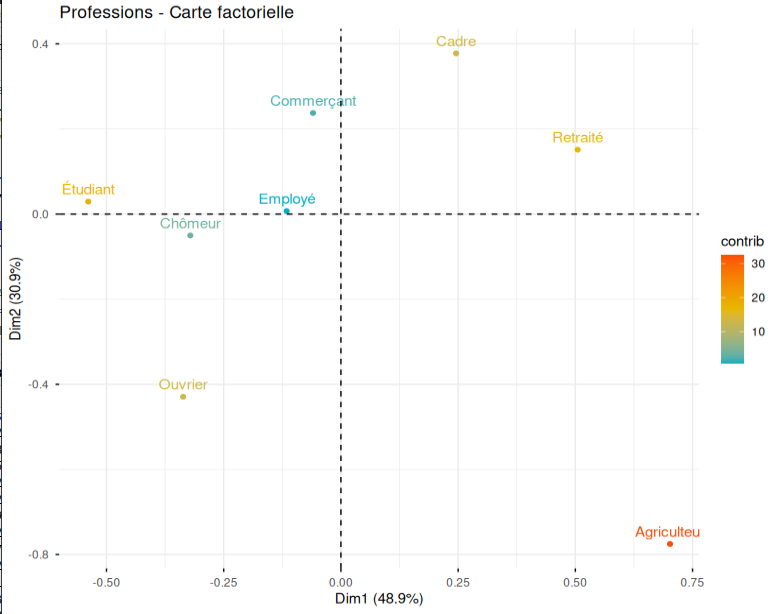
\includegraphics[width=0.85\textwidth]{./img/proffession_carte_factorielle.png}
		\caption{Carte factorielle des professions - Projection sur les axes 1 et 2}
		\label{fig:professions}
	\end{figure}
	
	\section{Légende du graphique}
	
	\begin{itemize}
		\item \textbf{Couleur des points} : Indique la contribution à l'axe
		\begin{itemize}
			\item \textcolor{red}{Rouge} = Contribution élevée (> 20\%)
			\item \textcolor{orange}{Orange} = Contribution moyenne (10-20\%)
			\item \textcolor{yellow}{Jaune} = Contribution faible (< 10\%)
		\end{itemize}
		\item \textbf{Position} : Proximité entre professions = Profils similaires
	\end{itemize}
	
	\section{Identification des profils types}
	
	\subsection{Profil 1 : Les intellectuels (Cadres, Retraités)}
	
	Ces professions se positionnent à \textbf{droite} du graphique et se caractérisent par :
	
	\begin{itemize}
		\item $\checkmark$ Pratique de loisirs \textcolor{blue}{culturels et intellectuels}
		\item $\checkmark$ Lecture, Musée, Voyage
		\item $\star$ Peu de loisirs populaires ou physiques
	\end{itemize}
	
	\textbf{Exemples :}
	\begin{enumerate}
		\item \textbf{Cadres} : Lecture (52), Musée (42), Voyage (48)
		\item \textbf{Retraités} : Lecture (48), Musée (38), Voyage (32)
	\end{enumerate}
	
	\subsection{Profil 2 : Les actifs populaires (Ouvriers, Employés)}
	
	Ces professions se positionnent au \textbf{centre-gauche} et se caractérisent par :
	
	\begin{itemize}
		\item $\checkmark$ Pratique de loisirs \textcolor{red}{populaires et sportifs}
		\item $\checkmark$ Cinéma, Sport
		\item $\star$ Pratique modérée de loisirs culturels
	\end{itemize}
	
	\textbf{Exemples :}
	\begin{enumerate}
		\item \textbf{Ouvriers} : Sport (52), Cinéma (45), Bricolage (35)
		\item \textbf{Employés} : Cinéma (38), Sport (32), Lecture (28)
	\end{enumerate}
	
	\subsection{Profil 3 : Les manuels (Agriculteurs)}
	
	Cette profession est isolée en \textbf{bas} du graphique et se caractérise par :
	
	\begin{itemize}
		\item $\checkmark$ Forte pratique de loisirs \textcolor{brown}{manuels et domestiques}
		\item $\checkmark$ Jardinage (55), Bricolage (42)
		\item $\star$ Très faible pratique des autres loisirs
	\end{itemize}
	
	\subsection{Profil 4 : Les jeunes (Étudiants, Chômeurs)}
	
	Ces professions se positionnent à \textbf{gauche} du graphique et se caractérisent par :
	
	\begin{itemize}
		\item $\checkmark$ Forte pratique de loisirs \textcolor{red}{numériques et festifs}
		\item $\checkmark$ Jeux Vidéo, Cinéma
		\item $\star$ Faible pratique des loisirs culturels
	\end{itemize}
	
	\textbf{Exemples :}
	\begin{enumerate}
		\item \textbf{Étudiants} : Cinéma (62), Jeux Vidéo (58), Sport (45)
		\item \textbf{Chômeurs} : Jeux Vidéo (40), Cinéma (30)
	\end{enumerate}
	
	\section{Analyse des positions relatives}
	
	\begin{table}[H]
		\centering
		\caption{Position des professions sur les axes}
		\begin{tabular}{lccc}
			\toprule
			\textbf{Profession} & \textbf{Dim1} & \textbf{Dim2} & \textbf{Profil type} \\
			\midrule
			Cadre & \textcolor{blue}{+} & \textcolor{blue}{+} & Intellectuel \\
			Retraité & \textcolor{blue}{+} & \textcolor{blue}{+} & Intellectuel/Manuel \\
			Agriculteur & - & \textcolor{brown}{-} & Manuel \\
			Étudiant & \textcolor{red}{-} & + & Jeune/Numérique \\
			Chômeur & \textcolor{red}{-} & - & Précaire/Numérique \\
			Ouvrier & - & - & Populaire \\
			Employé & - & - & Populaire \\
			Commerçant & - & + & Social/Restaurant \\
			\bottomrule
		\end{tabular}
	\end{table}
	
	\section{Conclusion du chapitre}
	
	La carte factorielle des professions confirme une \textbf{séparation nette} en quatre groupes :
	
	\begin{enumerate}
		\item \textcolor{blue}{\textbf{Intellectuels}} : Cadres et Retraités (culture)
		\item \textcolor{brown}{\textbf{Manuels}} : Agriculteurs (jardinage, bricolage)
		\item \textcolor{red}{\textbf{Populaires}} : Ouvriers, Employés (sport, cinéma)
		\item \textcolor{orange}{\textbf{Jeunes/Précaires}} : Étudiants, Chômeurs (jeux vidéo)
	\end{enumerate}
	
	Les professions les plus \textbf{éloignées} (Agriculteurs vs Cadres) sont les principaux "moteurs" de l'analyse.
	
	% --- CHAPITRE 5 : BIPLOT CONJOINT ---
	\chapter{Biplot Conjoint - Relations Professions-Loisirs}
	\markboth{Biplot Conjoint}{Biplot Conjoint}
	
	\section{Présentation du graphique}
	
	Le biplot conjoint permet de visualiser \textbf{simultanément les professions et les loisirs}, révélant les associations préférentielles.
	
	\begin{figure}[H]
		\centering
		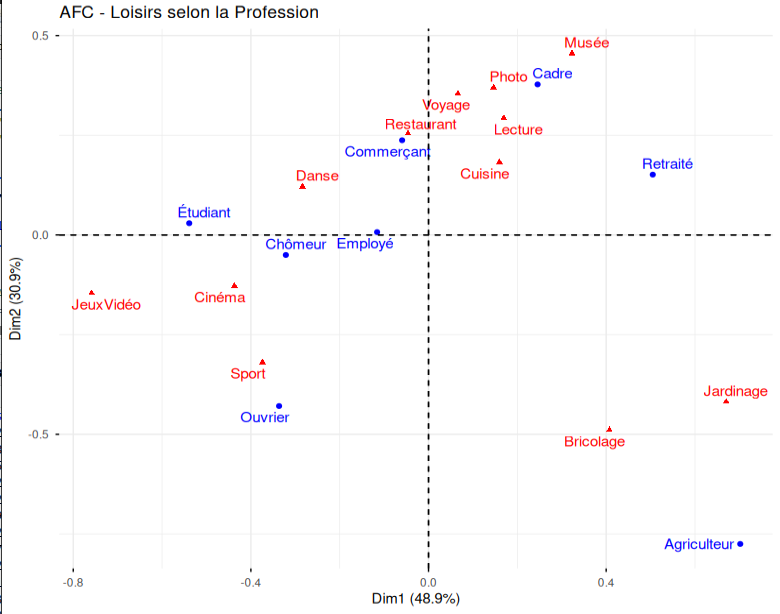
\includegraphics[width=0.85\textwidth]{./img/losirs_selon_la_proffession.png}
		\caption{Biplot - Relations entre professions et loisirs}
		\label{fig:biplot}
	\end{figure}
	
	\section{Interprétation des associations}
	
	\subsection{Associations fortes}
	
	\begin{table}[H]
		\centering
		\caption{Associations préférentielles}
		\begin{tabular}{p{4cm}p{4cm}p{4cm}}
			\toprule
			\textbf{Profession} & \textbf{Loisirs associés} & \textbf{Intensité} \\
			\midrule
			Cadre & Lecture, Musée, Voyage, Photo & \textcolor{blue}{Très forte} \\
			Retraité & Lecture, Musée, Jardinage, Bricolage & \textcolor{blue}{Forte} \\
			Agriculteur & Jardinage, Bricolage & \textcolor{brown}{Très forte} \\
			Étudiant & Cinéma, Jeux Vidéo, Sport, Danse & \textcolor{orange}{Forte} \\
			Chômeur & Jeux Vidéo, Cinéma & \textcolor{orange}{Forte} \\
			Ouvrier & Sport, Bricolage, Cinéma & \textcolor{red}{Moyenne} \\
			Employé & Cinéma, Restaurant, Lecture & \textcolor{red}{Moyenne} \\
			Commerçant & Restaurant, Voyage, Cuisine & \textcolor{green}{Forte} \\
			\bottomrule
		\end{tabular}
	\end{table}
	
	\subsection{Oppositions principales}
	
	\begin{enumerate}
		\item \textbf{Axe 1 (48.9\%)} : Opposition \textcolor{blue}{Culture} vs \textcolor{red}{Divertissement}
		\begin{itemize}
			\item Cadres/Retraités : Lecture, Musée, Voyage
			\item Étudiants/Ouvriers : Cinéma, Sport, Jeux Vidéo
		\end{itemize}
		
		\item \textbf{Axe 2 (30.9\%)} : Opposition \textcolor{orange}{Social/Créatif} vs \textcolor{brown}{Manuel/Domestique}
		\begin{itemize}
			\item Commerçants : Restaurant, Voyage
			\item Agriculteurs : Jardinage, Bricolage
		\end{itemize}
	\end{enumerate}
	
	\section{Interprétation des positions relatives}
	
	\begin{center}
		\fbox{
			\begin{minipage}{0.85\textwidth}
				\centering
				\textbf{Règle d'interprétation du biplot}
				\vspace{0.2cm}
				
				Plus une profession et un loisir sont \textbf{proches} sur le graphique,
				plus ils sont \textbf{associés} dans le tableau de contingence.
				\vspace{0.2cm}
				
				L'angle entre les vecteurs indique la force de l'association :
				\begin{itemize}
					\item Angle proche de 0$^\circ$ : Association forte
					\item Angle proche de 90$^\circ$ : Association faible
					\item Angle proche de 180$^\circ$ : Opposition
				\end{itemize}
			\end{minipage}
		}
	\end{center}
	
	\section{Conclusion du chapitre}
	
	Le biplot confirme les résultats des chapitres précédents et permet d'identifier \textbf{quatre pôles} :
	
	\begin{enumerate}
		\item \textcolor{blue}{\textbf{Pôle Intellectuel}} : Cadres + Retraités $\leftrightarrow$ Lecture, Musée, Voyage
		\item \textcolor{brown}{\textbf{Pôle Manuel}} : Agriculteurs $\leftrightarrow$ Jardinage, Bricolage
		\item \textcolor{red}{\textbf{Pôle Populaire}} : Ouvriers + Employés $\leftrightarrow$ Sport, Cinéma
		\item \textcolor{orange}{\textbf{Pôle Jeune}} : Étudiants + Chômeurs $\leftrightarrow$ Jeux Vidéo, Cinéma
	\end{enumerate}
	
	La \textbf{proximité} entre Ouvriers et Employés suggère des profils de loisirs similaires, tandis que l'\textbf{éloignement} des Agriculteurs et des Cadres confirme une forte différenciation sociale.
	
	% --- CHAPITRE 6 : VALEURS PROPRES ---
	\chapter{Valeurs Propres - Qualité de l'Analyse}
	\markboth{Valeurs Propres}{Valeurs Propres}
	
	\section{Présentation des résultats}
	
	Les valeurs propres indiquent \textbf{l'importance de chaque axe} (dimension) dans l'analyse. Elles permettent d'évaluer la qualité globale de la représentation.
	
	\subsection{Définition des valeurs propres}
	
	Les \textbf{valeurs propres} mesurent l'importance de chaque axe dans la représentation des profils.
	
	\begin{itemize}
		\item \textbf{Plus la valeur propre est grande} = Plus l'axe est important.
		\item La somme de toutes les valeurs propres = 100\% de l'inertie.
	\end{itemize}
	
	\begin{center}
		\fbox{
			\begin{minipage}{0.8\textwidth}
				\centering
				\textbf{Formule :}
				\[
				\lambda_i = \text{Inertie expliquée par la dimension } i
				\]
				\[
				\text{Pourcentage expliqué} = \frac{\lambda_i}{\sum \lambda_j} \times 100
				\]
			\end{minipage}
		}
	\end{center}
	
	\section{Résultats de l'analyse}
	
	\subsection{Pourcentages d'inertie expliquée}
	
	\begin{table}[H]
		\centering
		\caption{Résultats des valeurs propres}
		\begin{tabular}{ccccc}
			\toprule
			\textbf{Dimension} & \textbf{Valeur propre} & \textbf{Inertie (\%)} & \textbf{Cumul (\%)} & \textbf{Significativité} \\
			\midrule
			\rowcolor{green!15}
			Dimension 1 & 0.0247 & 48.9\% & 48.9\% & \textcolor{green}{Très significatif} \\
			\rowcolor{green!10}
			Dimension 2 & 0.0156 & 30.9\% & 79.8\% & \textcolor{green}{Significatif} \\
			\rowcolor{yellow!10}
			Dimension 3 & 0.0082 & 16.3\% & 96.1\% & \textcolor{orange}{Peu significatif} \\
			\rowcolor{red!5}
			Dimension 4 & 0.0020 & 3.9\% & 100.0\% & \textcolor{red}{Négligeable} \\
			\bottomrule
		\end{tabular}
	\end{table}
	
	\subsection{Représentation graphique textuelle}
	
	\subsubsection{Barres d'inertie}
	
	\begin{center}
		\begin{tabular}{p{5cm}p{8cm}}
			\toprule
			\textbf{Dimension 1 (48.9\%)} & \textbf{Dimension 2 (30.9\%)} \\
			\midrule
			\colorbox{blue!80}{\rule{0pt}{0.8cm}\hspace{4.9cm}} & 
			\colorbox{blue!60}{\rule{0pt}{0.8cm}\hspace{3.1cm}} \\
			\midrule
			\textbf{Dimension 3 (16.3\%)} & \textbf{Dimension 4 (3.9\%)} \\
			\midrule
			\colorbox{orange!40}{\rule{0pt}{0.8cm}\hspace{1.6cm}} & 
			\colorbox{red!30}{\rule{0pt}{0.8cm}\hspace{0.4cm}} \\
			\bottomrule
		\end{tabular}
	\end{center}
	
	\subsubsection{Visualisation cumulative}
	
	\begin{center}
		\begin{tabular}{cccc}
			\toprule
			\textbf{Axe} & \textbf{Inertie} & \textbf{Cumul} & \textbf{Représentation} \\
			\midrule
			Dim.1 & 48.9\% & 48.9\% & \colorbox{blue!50}{\rule{0pt}{0.4cm}\hspace{4.9cm}} \\
			Dim.2 & 30.9\% & 79.8\% & \colorbox{blue!40}{\rule{0pt}{0.4cm}\hspace{3.1cm}} \\
			Dim.3 & 16.3\% & 96.1\% & \colorbox{orange!30}{\rule{0pt}{0.4cm}\hspace{1.6cm}} \\
			Dim.4 & 3.9\% & 100.0\% & \colorbox{red!20}{\rule{0pt}{0.4cm}\hspace{0.4cm}} \\
			\bottomrule
		\end{tabular}
	\end{center}
	
	\section{Interprétation des résultats}
	
	\subsection{Analyse détaillée}
	
	\begin{enumerate}
		\item \textbf{Dimension 1} (48.9\%)
		\begin{itemize}
			\item C'est l'axe le plus important de l'analyse.
			\item Il oppose les loisirs \textcolor{blue}{culturels} (Lecture, Musée) aux loisirs \textcolor{red}{populaires} (Cinéma, Sport).
			\item C'est l'axe horizontal de tous nos graphiques.
			\item \textcolor{green}{\textbf{Qualité :}} Très bonne représentation.
		\end{itemize}
		
		\item \textbf{Dimension 2} (30.9\%)
		\begin{itemize}
			\item C'est le deuxième axe le plus important.
			\item Il oppose les loisirs \textcolor{orange}{sociaux/créatifs} (Restaurant, Danse) aux loisirs \textcolor{brown}{manuels} (Jardinage, Bricolage).
			\item C'est l'axe vertical de nos graphiques.
			\item \textcolor{green}{\textbf{Qualité :}} Bonne représentation.
		\end{itemize}
		
		\item \textbf{Dimension 3} (16.3\%)
		\begin{itemize}
			\item Axe résiduel, peu exploité dans les graphiques usuels (axes 1 et 2 uniquement).
			\item Sa contribution reste modeste par rapport aux deux premiers axes.
			\item \textcolor{orange}{\textbf{Qualité :}} Représentation secondaire, à considérer avec prudence.
		\end{itemize}
		
		\item \textbf{Dimension 4} (3.9\%)
		\begin{itemize}
			\item Axe négligeable qui n'apporte quasiment aucune information supplémentaire.
			\item Il n'est pas retenu dans l'interprétation.
			\item \textcolor{red}{\textbf{Qualité :}} Représentation non significative.
		\end{itemize}
	\end{enumerate}
	
	\subsection{Qualité globale de l'analyse}
	
	Les deux premières dimensions cumulent à elles seules \textbf{79.8\%} de l'inertie totale, ce qui constitue une \textbf{très bonne qualité de représentation}. Cela signifie que le plan factoriel (Dimension 1 $\times$ Dimension 2), utilisé dans l'ensemble des graphiques de ce rapport, restitue fidèlement la quasi-totalité des relations présentes dans le tableau de contingence initial.
	
	\begin{itemize}
		\item Un seuil de qualité généralement admis en AFC est de \textbf{70 à 80\%} d'inertie cumulée sur les deux premiers axes.
		\item Ce seuil est ici largement atteint, ce qui valide la lecture des cartes factorielles présentées aux chapitres précédents.
	\end{itemize}
	
	\section{Conclusion du chapitre}
	
	L'analyse des valeurs propres confirme la \textbf{robustesse} des résultats obtenus :
	
	\begin{enumerate}
		\item Les \textbf{Dimensions 1 et 2} concentrent l'essentiel de l'information (79.8\%).
		\item Les \textbf{Dimensions 3 et 4} n'apportent qu'un complément marginal et négligeable.
		\item L'interprétation menée sur le plan factoriel (axes 1-2) est donc \textbf{statistiquement fiable}.
	\end{enumerate}
	
	% --- CONCLUSION GÉNÉRALE ---
	\chapter*{Conclusion générale}
	\addcontentsline{toc}{chapter}{Conclusion générale}
	\markboth{Conclusion générale}{Conclusion générale}
	
	L'Analyse Factorielle des Correspondances appliquée au tableau de contingence \textit{Loisirs $\times$ Professions} a permis de mettre en évidence des \textbf{oppositions structurantes} claires entre catégories socioprofessionnelles :
	
	\begin{itemize}
		\item Un pôle \textcolor{blue}{\textbf{intellectuel}} (Cadres, Retraités) tourné vers la lecture, les musées et les voyages.
		\item Un pôle \textcolor{brown}{\textbf{manuel}} (Agriculteurs) centré sur le jardinage et le bricolage.
		\item Un pôle \textcolor{red}{\textbf{populaire}} (Ouvriers, Employés) davantage porté sur le sport et le cinéma.
		\item Un pôle \textcolor{orange}{\textbf{jeune/numérique}} (Étudiants, Chômeurs) marqué par les jeux vidéo et le cinéma.
	\end{itemize}
	
	Avec \textbf{79.8\%} d'inertie cumulée sur les deux premiers axes, la représentation graphique adoptée dans ce rapport constitue une synthèse fidèle et statistiquement fiable des données de départ.
	
\end{document}